\subsection{Exercise 1}
\begin{figure}[H]
    \centering
    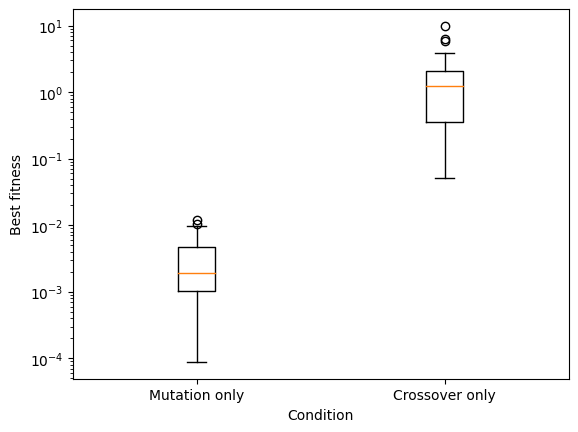
\includegraphics[width=\linewidth]{images/lab2/no_cross_no_mut.png}
\end{figure}
\begin{lstlisting}
Average fitness for mutation only: 0.003610780363409824
Average fitness for crossover only: 1.8424724971346327
\end{lstlisting}
Using crossover only we don't introduce any new genetic material but simply recombine the one already available (exploitation) while with mutations we vary the solutions we have (exploration).This means that a genetic algorithm using crossover only is strongly related to how the original population is initialized since no new information are introduced while mutation only processes rely on the randomness of the mutation to be a mutation that betters the fitness. The best solution is usually to use a combination of the two where the probabilities of each one depend on the shape of the fitness landscape.

\subsection{Exercise 2}
\begin{figure}[H]
    \centering
    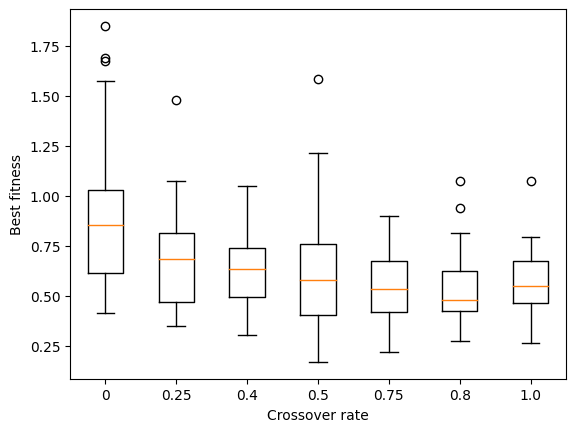
\includegraphics[width=\linewidth]{images/lab2/comp_cross.png}
\end{figure}
We can see that the best fitness value is obtained with a quite high crossover rate (around 0.8). Having a very low crossover rate means that we don't exploit the combination of the parents while a too high crossover rate means that there is a larger probability that the crossover of a large number of genomes "disrupts" the genome too much and gives us a worse offspring than both of its parents.

Moreover, the crossover is evaluated of the sphere function (the fitness function is the squared sum of the genes) and thus different fitness function may lead to different optimal crossover rates

\subsection{Exercise 3}
\begin{figure}[H]
    \centering
    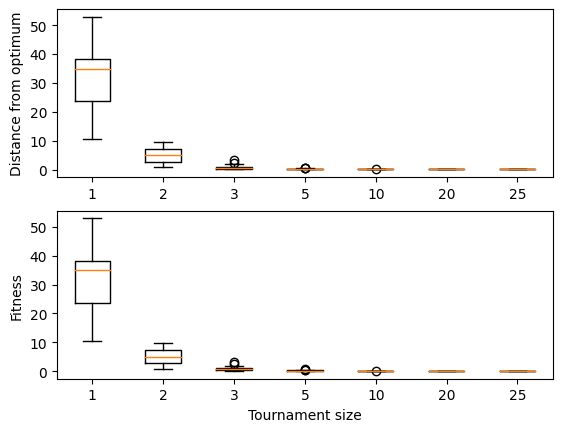
\includegraphics[width=\linewidth]{images/lab2/tournament_sphere.png}
\end{figure}
Being the Sphere function unimodal it makes sense that larger tournaments, where the selection pressure is higher, are better since the point with lower fitness is closer to a minima that we know is the global minima.

\begin{figure}[H]
    \centering
    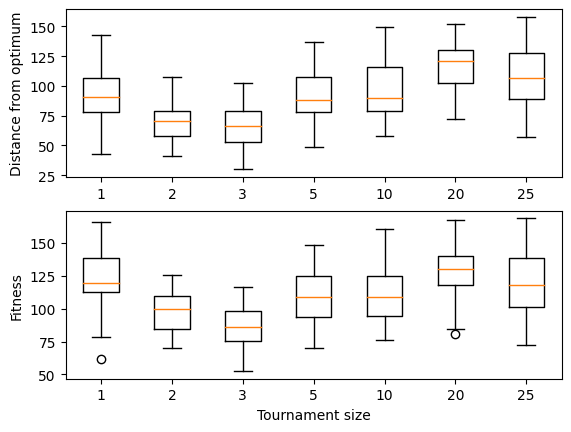
\includegraphics[width=\linewidth]{images/lab2/tournament_rastrigin.png}
\end{figure}
Harder function to optimize, even fine tuning the tournament size we don't have a great fitness value

\subsection{Exercise 4}
\subsubsection{Sphere}
Description of Sphere function
\begin{figure}[H]
    \centering
    \begin{subfigure}[t]{0.5\textwidth}
        \centering
        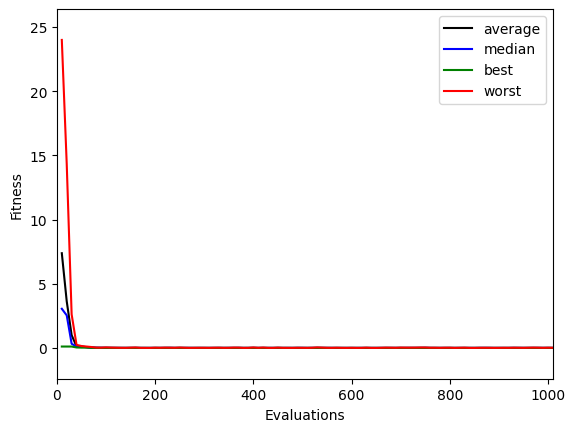
\includegraphics[width=\linewidth]{images/lab2/sphere_eval.png}
    \end{subfigure}%
    \begin{subfigure}[t]{0.5\textwidth}
        \centering
        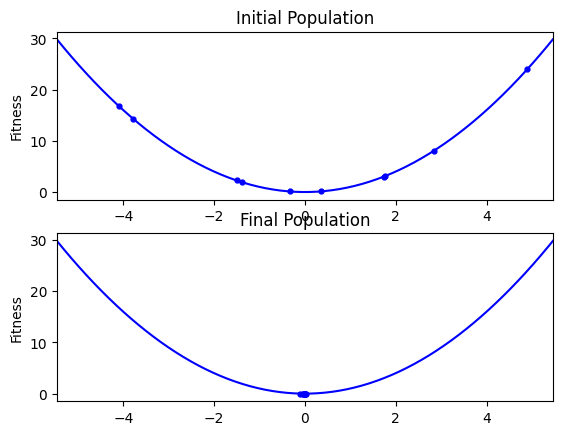
\includegraphics[width=\linewidth]{images/lab2/sphere_pop.png}
    \end{subfigure}
\end{figure}
Easy function to reach the minimum, only difference from default parameters is a smaller standard deviation (0.1) to have smaller mutations

\subsubsection{Griewank}
From now on all evolutions are done on a population of 25 individuals instead of the default 10
\begin{figure}[H]
    \centering
    \begin{subfigure}[t]{0.5\textwidth}
        \centering
        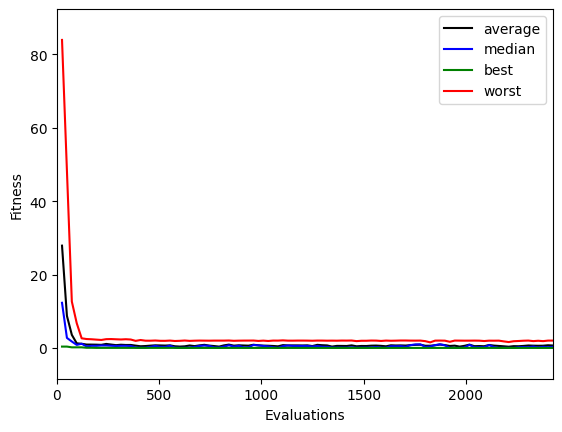
\includegraphics[width=\linewidth]{images/lab2/grie_eval.png}
    \end{subfigure}%
    \begin{subfigure}[t]{0.5\textwidth}
        \centering
        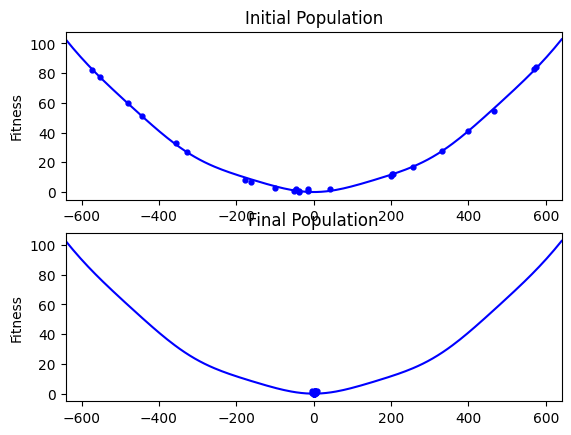
\includegraphics[width=\linewidth]{images/lab2/grie_pop.png}
    \end{subfigure}
\end{figure}
Even if it's multimodal, the function is simple enough that it's basically the same thing as running the algorithm for the sphere function.

\subsubsection{Ackley}
\begin{figure}[H]
    \centering
    \begin{subfigure}[t]{0.5\textwidth}
        \centering
        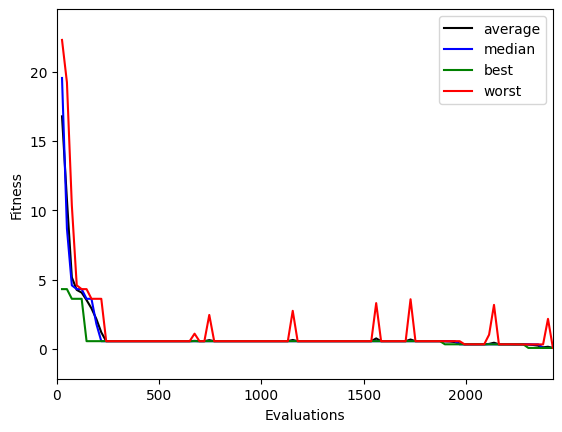
\includegraphics[width=\linewidth]{images/lab2/ack_eval.png}
    \end{subfigure}%
    \begin{subfigure}[t]{0.5\textwidth}
        \centering
        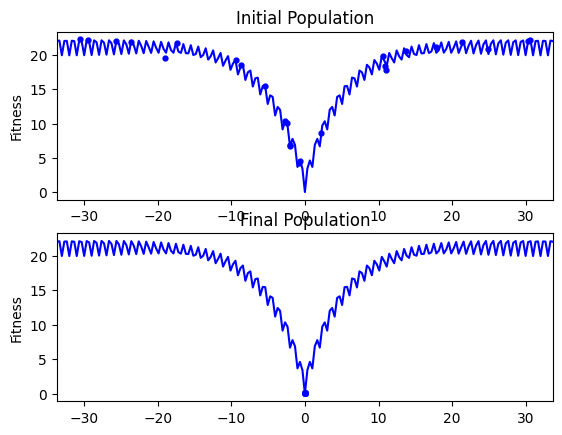
\includegraphics[width=\linewidth]{images/lab2/ack_pop.png}
    \end{subfigure}
\end{figure}
Being the function multimodal but still with a pronounced global minimum, we don't need much exploration of the fitness landscape (once we see that the fitness function decreases by a big amount we know we're moving closer to the global minimum) so use parameters that penalize diversity (low mutation rate (0.1) and an elitist approach (5 best parents for generation)

\subsubsection{Rastring}
\begin{figure}[H]
    \centering
    \begin{subfigure}[t]{0.5\textwidth}
        \centering
        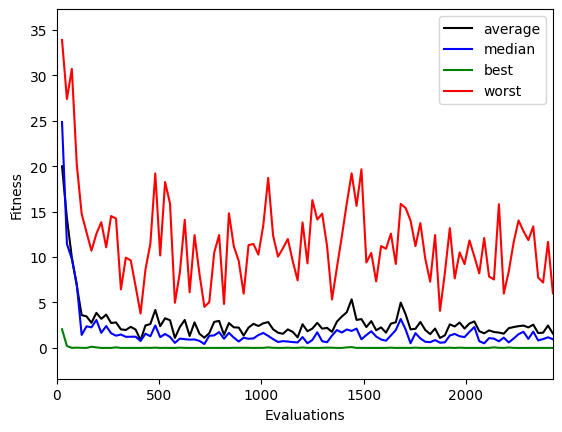
\includegraphics[width=\linewidth]{images/lab2/rast_eval.png}
    \end{subfigure}%
    \begin{subfigure}[t]{0.5\textwidth}
        \centering
        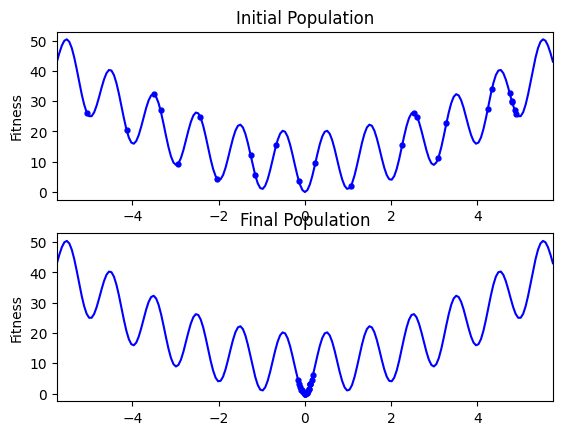
\includegraphics[width=\linewidth]{images/lab2/rast_pop.png}
    \end{subfigure}
\end{figure}
We use an approach more skewed towards mutation than crossover (0.9 mutation rate with standrd deviation 0.1 and 0.3 crossover rate) in order to help get out of the local minima close to the global one (to help in this we also choose to have no parents from the previous generation survive). Even with this for some cases we still don't reach the global minimum
\begin{figure}[H]
    \centering
    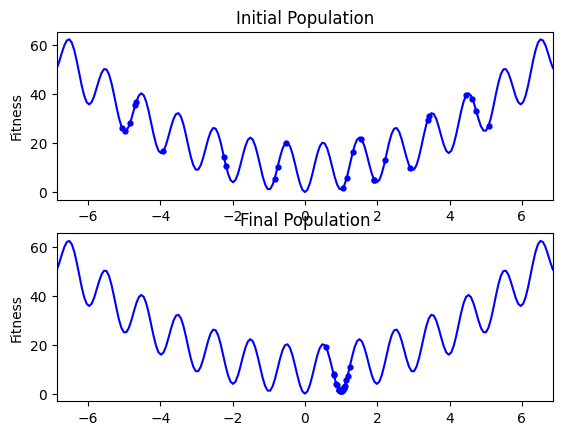
\includegraphics[width=\linewidth]{images/lab2/rast_err.png}
\end{figure}

\subsubsection{Schwefel}
\begin{figure}[H]
    \centering
    \begin{subfigure}[t]{0.5\textwidth}
        \centering
        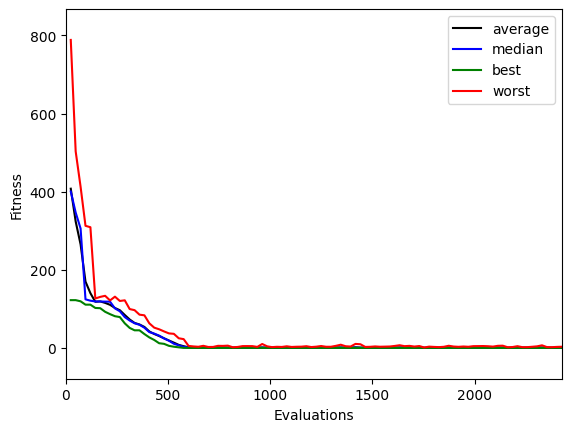
\includegraphics[width=\linewidth]{images/lab2/sch_eval.png}
    \end{subfigure}%
    \begin{subfigure}[t]{0.5\textwidth}
        \centering
        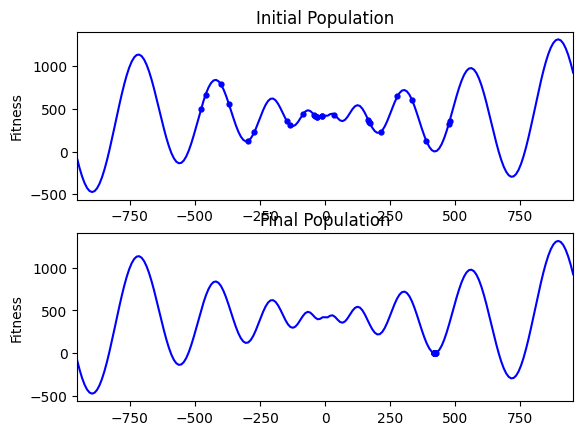
\includegraphics[width=\linewidth]{images/lab2/sch_pop.png}
    \end{subfigure}
\end{figure}
There is a condition of early convergence as the points all converge in the non global minima and lose diversity

\subsection{General questions}
\begin{itemize}
    \item Why is it useful to introduce crossover in EA? Can you think of any cases when mutation only can work effectively, without crossover? What about using crossover only, without mutation? Crossover allows to use the genetic material we already have in our genes and combine it trying to find a better offspring that is better than both its parents. While we can find the global optimum using only mutations if we have enough generations simply by luck, it's much harder to find the minimum using crossover only as no new genetic information is introduced, only scrambled around and thus possible convergence is mainly dependent on the initialization conditions.
    
    \item What's the effect of changing the fraction of offspring created by crossover? We reduce how much the offspring interacts and thus the possibility of creating better offspring by combining two suboptimal solution 
    
    \item Are there optimal parameters for an EA? No, there are no optimal parameters that work for all landscapes given how much they differ (NFL theorem).
    
    \item What are the advantages and disadvantages of low/high selection pressure? Having an lower selection pressure (at the extreme random selection) means not caring too much about the fitness value and giving parents with not great fitness the opportunity to have offspring (thus giving more importance to exploration) while an high selection pressure means only selecting the best parent we already have (exploitation over exploration). An easy way to find a tradeoff between the two is using the tournament selection. 
\end{itemize}